% ADD/REMOVE THE 'answers' OPTION TO INCLUDE/SUPPRESS SOLUTIONS
%\documentclass[11pt,addpoints]{exam}
\documentclass[11pt,addpoints,answers]{exam}

\newcommand{\hwnum}{2}
\newcommand{\duedate}{September 16}

% In order to compile this file you will need to get 'header.tex'
% and make the line below point to the appropriate file path
\RequirePackage{microtype}
\RequirePackage{mathtools}
\RequirePackage{amsthm}
\RequirePackage{amssymb}
\RequirePackage{xspace}
\RequirePackage[shortlabels]{enumitem}
\RequirePackage{xcolor}
\RequirePackage{hyperref}
\RequirePackage[capitalize,nameinlink,noabbrev]{cleveref} % must load after hyperref
\usepackage{fvextra} % To use Verbatim
\usepackage{diagbox} % For diagbox
\RequirePackage[boxed]{algorithm}
\RequirePackage[noend]{algpseudocode}
\RequirePackage{tikz}
\usetikzlibrary{arrows,automata,positioning}

\hypersetup{breaklinks=true,
    colorlinks=true,
    linkcolor=blue,
    filecolor=blue,
    citecolor=blue,
    urlcolor=blue}

\algrenewcommand{\algorithmiccomment}[1]{\texttt{//} #1}
\algrenewcommand\algorithmicrequire{\textbf{Input:}}
\algrenewcommand\algorithmicensure{\textbf{Output:}}


% allow cleveref to label and reference enumerables defined in the exam class.
% these automatically define corresponding \Crefname as well.

% https://tex.stackexchange.com/questions/126020/cleveref-doesnt-use-correct-capitalized-name-if-used-with-amsthm
\makeatletter
\if@cref@capitalise
\crefname{question}{Question}{Questions}
\Crefname{partno}{Part}{Parts}
\crefname{subpart}{Subpart}{Subparts)}
\crefname{subsubpart}{Subsubpart}{Subsubparts}
\else
\crefname{question}{question}{questions}
\crefname{partno}{part}{parts}
\crefname{subpart}{subpart}{subparts}
\crefname{subsubpart}{subsubpart}{subsubparts}
\fi
\makeatother

% numeric sets in "blackboard" font

\newcommand{\N}{\mathbb{N}}
\newcommand{\Z}{\mathbb{Z}}
\newcommand{\R}{\mathbb{R}}
\newcommand{\Q}{\mathbb{Q}}
\newcommand{\C}{\mathbb{C}}
\newcommand{\Prop}{\mathbb{P}}

% paired delimiters

\DeclarePairedDelimiter\abs{\lvert}{\rvert}
\DeclarePairedDelimiter\length{\lVert}{\rVert}
\DeclarePairedDelimiter\norm{\lVert}{\rVert}
\DeclarePairedDelimiter\parens{(}{)}
\DeclarePairedDelimiter\tuple{(}{)}
\DeclarePairedDelimiter\brackets{[}{]}
\DeclarePairedDelimiter\floor{\lfloor}{\rfloor}
\DeclarePairedDelimiter\ceil{\lceil}{\rceil}
\DeclarePairedDelimiter\round{\lfloor}{\rceil}
\DeclarePairedDelimiter\set{\{}{\}}
\DeclarePairedDelimiter\inner{\langle}{\rangle}

\newcommand{\bit}{\set{0,1}}

% asymptotics

\DeclareMathOperator{\Otil}{\tilde{O}}
\DeclareMathOperator{\poly}{poly}
\DeclareMathOperator{\polylog}{polylog}
\DeclareMathOperator{\negl}{negl}

% algorithms

\newcommand{\algo}[1]{\textsc{#1}}

\newcommand{\memo}{\text{memo}}
\newcommand{\tabl}{\text{table}}
\newcommand{\backtrack}{\text{backtrack}}

\newcommand{\ALG}{\text{ALG}}
\newcommand{\OPT}{\text{OPT}}
\newcommand{\weight}{\text{weight}}
\newcommand{\val}{\text{value}}

% computability

% named language
\newcommand{\lang}[1]{L_{\text{#1}}}
% computational problem
\newcommand{\cproblem}[1]{\ensuremath{\text{#1}}\xspace}
% class of languages
\newcommand{\class}[1]{\ensuremath{\mathsf{#1}}\xspace}

\newcommand{\qst}{q_{\text{start}}}
\newcommand{\qacc}{q_{\text{acc}}}
\newcommand{\qrej}{q_{\text{rej}}}

\newcommand{\Lbarber}{\lang{BARBER}}
\newcommand{\atm}{\lang{ACC}}
\newcommand{\htm}{\lang{HALT}}
\newcommand{\ehtm}{\lang{$\varepsilon$-HALT}}
\newcommand{\eqtm}{\lang{EQ}}
\newcommand{\etm}{\lang{$\emptyset$}}
\newcommand{\epstm}{\lang{$\set{\varepsilon}$}}
\newcommand{\Lprop}{\lang{$\Prop$}}
\newcommand{\LSigmastar}{\lang{$\Sigma^*$}}

% complexity

\newcommand{\yes}{\ensuremath{\text{YES}}}
\newcommand{\no}{\ensuremath{\text{NO}}}

\newcommand{\DTIME}{\class{DTIME}}
\renewcommand{\P}{\class{P}}
\newcommand{\NP}{\class{NP}}
\newcommand{\NPH}{\class{NPH}}
\newcommand{\NPC}{\class{NPC}}
\newcommand{\coNP}{\class{coNP}}

\newcommand{\MAZE}{\cproblem{MAZE}}
\newcommand{\PALINDROME}{\cproblem{PALINDROME}}
\newcommand{\TSP}{\cproblem{TSP}}
\newcommand{\SAT}{\cproblem{SAT}}
\newcommand{\CSAT}{\cproblem{CSAT}}
\newcommand{\TSAT}{\cproblem{3SAT}}
\newcommand{\VC}{\cproblem{VERTEX-COVER}}
\newcommand{\DS}{\cproblem{DOMINATING-SET}}
\newcommand{\SC}{\cproblem{SET-COVER}}
\newcommand{\HC}{\cproblem{HAMCYCLE}}
\newcommand{\HP}{\cproblem{HAMPATH}}
\newcommand{\AHP}{\cproblem{ANYHAMPATH}}
\newcommand{\IS}{\cproblem{IS}}
\newcommand{\CLIQUE}{\cproblem{CLIQUE}}
\newcommand{\SSUM}{\cproblem{SUBSET-SUM}}
\newcommand{\KNAPSACK}{\cproblem{KNAPSACK}}
\newcommand{\MAXCUT}{\cproblem{MAX-CUT}}

% randomness

\DeclareMathOperator*{\Var}{Var}
\DeclareMathOperator*{\Ex}{\mathbb{E}}

\newcommand{\RP}{\class{RP}}
\newcommand{\coRP}{\class{coRP}}
\newcommand{\BPP}{\class{BPP}}
\newcommand{\ZPP}{\class{ZPP}}
\newcommand{\BQP}{\class{BQP}}

%%% misc

\newcommand{\eps}{\varepsilon}

%%% theorems

\theoremstyle{plain}            % following are "theorem" style

\newtheorem{theorem}{Theorem}
\newtheorem{lemma}[theorem]{Lemma}
\newtheorem{corollary}[theorem]{Corollary}
\newtheorem{proposition}[theorem]{Proposition}
\newtheorem{claim}[theorem]{Claim}
\newtheorem{fact}[theorem]{Fact}
\newtheorem{openproblem}[theorem]{Open Problem}

\theoremstyle{definition}       % following are def style

\newtheorem{definition}[theorem]{Definition}
\newtheorem{conjecture}[theorem]{Conjecture}
\newtheorem{protocol}[theorem]{Protocol}
\newtheorem{exercise}[theorem]{Exercise}

\theoremstyle{remark}           % following are remark style

\newtheorem{example}[theorem]{Example}
\newtheorem{remark}[theorem]{Remark}
\newtheorem{note}[theorem]{Note}

%%% for homework and section notes

\newcommand{\commonheader}[2]{
    \pagestyle{headandfoot}
    \setlength{\headheight}{26pt}
    \setlength{\headsep}{16pt}

    \header
        {\small{\textbf{EECS 376: Foundations of Computer Science}} \\ \footnotesize{\textbf{University of Michigan, Fall 2026}}}
        {#1}
        {#2}

    \firstpageheadrule
    \runningheadrule

    \footer
        {}
        {\thepage}
        {}
}

\newcommand{\hwheader}{
    \commonheader
        {\Large \textbf{Homework \hwnum}}
        {\small \textbf{Due 8:00pm, \duedate\\ {\tiny(accepted until 10:00 pm, no credit after)}}}
}

\newcommand{\hwslnheader}{
    \commonheader
    	{}
        {\Large \textbf{Solutions to Homework \hwnum}}
    \printanswers
}

\newcommand{\notesheader}{
    \commonheader
    	{}
        {\Large \textbf{Discussion Notes \sectionnum}}
}

\newcommand{\practiceheader}{
    \commonheader
    	{}
        {\Large \textbf{Discussion Worksheet \sectionnum}}
}

\newcommand{\practiceslnheader}{
    \commonheader
    	{}
        {\Large \textbf{Solutions to Discussion Worksheet \sectionnum}}
}

\newcommand{\reviewheader}{
    \commonheader 
    \smallskip
    	{}
        {\Large \textbf{Midterm Review Notes}}
}

\newcommand{\hwpreface}{

\noindent This homework has \numquestions\ questions, for a total of \numpoints\ points and \numbonuspoints\ extra-credit points.

\noindent Unless otherwise stated, each question requires \emph{clear}, \emph{logically correct}, and \emph{sufficient} justification to convince the reader.

\noindent We strongly encourage you to typeset your solutions in \LaTeX.

}

\newcommand{\hint}[1]{
\emph{Hint}: #1
}

% exam class setup
\pointsinmargin
\pointpoints{pt}{pts}
\bonuspointpoints{EC pt}{EC pts}
\marginpointname{ \points}
\marginbonuspointname{ \bonuspoints}


\ifprintanswers
\hwslnheader   % header for solutions
\else
\hwheader   % header for homework
\fi

\DeclareMathOperator{\col}{color}

\begin{document}

% CAN REMOVE THIS BEFORE PUBLISHING SOURCE
\IfPackageLoadedTF{fixme}{\listoffixmes}{}

\hwpreface


\begin{questions}

  \addtocounter{question}{-1}
  \question[0] \textbf{Before you start; before you submit.} \nopagebreak

  \begin{parts}
    \part Before starting this assignment, carefully read \href{https://drive.google.com/file/d/1LzHBuS9pBCy12QMJ91PyLaDOnNW4NFn0/view?usp=drive_link}{Handout 3} about ``giving an algorithm,'' and follow it in your solutions.

    \part Correctness arguments and runtime analysis for divide-and-conquer/recursive algorithms should follow the recommended structure described in this week's discussion worksheet. 

    \part If applicable, state the name(s) and uniqname(s) of your collaborator(s).

    \begin{solution}
No collaborators.
\end{solution}

  \end{parts}

  \question[10] \textbf{Self assessment.} \nopagebreak
  Carefully read and understand the posted solutions to the previous homework.
  Identify one part for which your own solution has the most room for improvement (e.g., has unsound reasoning, doesn’t show what was required, could be significantly clearer or better organized, etc.).
  Copy or screenshot this solution, then in a few sentences, explain what was deficient and how it could be fixed.

  (Alternatively, if you think one of your solutions is significantly \emph{better} than the posted one, copy it here and explain why you think it is better.)

  If you didn't do last week's homework, choose a problem from it that looks challenging to you, and in a few sentences, explain the key ideas behind its solution in your own words.

  \begin{solution}
For the self-assessment, I would improve the clarity of my correctness arguments. In particular, I should state the key invariant explicitly and separate the initialization, preservation, and termination arguments. Doing this would make the logic easier to verify and would make it clearer why each step of the algorithm is valid.
\end{solution}

     \question \textbf{Recurrences.} \nopagebreak
  
  Define $T(n)= 9T(n/3) + O(g(n))$.
  With brief justification, apply the Master Theorem to derive a closed-form asymptotic (big-O) solution for $T(n)$ when $g(n)$ is each of the following:

  \begin{parts}
    \part[5] $g(n) = n^{3.5}$.

    \begin{solution}
We have \(a=9\) and \(b=3\), so
\[
n^{\log_b a}=n^{\log_3 9}=n^2.
\]
For \(g(n)=n^{3.5}\), \(g(n)=\Omega(n^{2+\varepsilon})\) with \(\varepsilon=1.5\). The regularity condition holds since
\[
9g(n/3)=9(n/3)^{3.5}=\frac{1}{3^{1.5}}n^{3.5}=O(g(n)).
\]
Thus Master Theorem Case 3 gives
\[
T(n)=O(n^{3.5}).
\]
\end{solution}
    
    \part[5] $g(n) = n\log n$.

    \begin{solution}
Again \(n^{\log_b a}=n^2\). We have
\[
n\log n=O(n^{2-\varepsilon})
\]
for example with \(\varepsilon=1/2\). Therefore Master Theorem Case 1 gives
\[
T(n)=O(n^2).
\]
\end{solution}
    
    \part[5] $g(n)= 5n^2$.

    \begin{solution}
Here
\[
g(n)=5n^2=\Theta(n^2)=\Theta\!\left(n^{\log_3 9}\right).
\]
Thus Master Theorem Case 2 applies, giving
\[
T(n)=O(n^2\log n).
\]
\end{solution}
  \end{parts}


 \question[15] \textbf{This is the pits.} \nopagebreak

  A \emph{pit} of an integer array $M[1,\ldots, n]$ is an element $M[i]$ that is no larger than its adjacent elements.
  More precisely, $M[i]$ is a pit if $M[i] \leq M[i-1]$ and $M[i] \leq M[i+1]$, where for convenience we say that $M[0] = M[n+1] = \infty$ to deal with the endpoints of the array.
  Note that by this definition, if~$M$ has just one element, then that element is a pit.
  Every array has at least one pit---namely, any smallest element in the array---though there may be others.
    
  A trivial algorithm can find the index of a pit of $M[1,\ldots,n]$ in $O(n)$ time.
  \textbf{Give an algorithm} to find the index of a pit in $O(\log n)$ time.
      
  \hint{Think about another $O(\log n)$-time algorithm you know that operates on one-dimensional arrays.}

   \textit{Note: Make sure you have read \href{https://drive.google.com/file/d/1LzHBuS9pBCy12QMJ91PyLaDOnNW4NFn0/view?usp=drive_link}{Handout 3} before attempting this question, and that you include all of the required parts.}
      
  \begin{solution}
Use a recursive binary-search-style algorithm. Given an interval \([l,r]\), let
\[
m=\left\lfloor\frac{l+r}{2}\right\rfloor.
\]
If \(M[m]\le M[m-1]\) and \(M[m]\le M[m+1]\), return \(m\). Otherwise, if \(M[m-1]<M[m]\), recursively search \([l,m-1]\); if \(M[m+1]<M[m]\), recursively search \([m+1,r]\). The comparisons with the outside values \(M[0]=M[n+1]=\infty\) handle endpoints.

If \(m\) is not a pit, at least one adjacent element is strictly smaller. Suppose \(M[m-1]<M[m]\). Consider the left interval \([l,m-1]\). Its right boundary neighbor in the original array is larger than its boundary element, so a minimum element of this interval is a pit in the original array. The same argument applies symmetrically when \(M[m+1]<M[m]\). Thus every recursive call contains a pit.

At each step the interval size is reduced by at least a constant factor, so
\[
T(n)=T(\lceil n/2\rceil)+O(1),
\]
and hence
\[
T(n)=O(\log n).
\]
\end{solution}



  \question \textbf{A hole different kind of tiling.} 

  Consider the following tiling problem: for some $n \geq 2$ that is a power of two, we want to tile an $n$-by-$n$ grid of unit squares using ``L-shaped'' tiles that are made up of three unit squares each.
  However, there is \emph{one designated} unit square in the grid that should remain \emph{uncovered}.
  The rest should be covered by tiles, without any overlap and with every tile contained entirely within the grid.
  The tiles may be oriented arbitrarily.

  See the diagram below for a small example of a four-by-four grid and the shape of the tile.
  The uncovered square is marked by a circle, and the thick right angles show the orientations of the tiles in a valid tiling.

  \begin{center}
    \begin{tikzpicture}
      \draw (0,0) grid (4,4);
      \begin{scope}[xshift=0.5cm,yshift=0.5cm]
        \fill (0,1) circle (5pt);
        \draw[very thick]
        (0,0) -| (1,1)
        (0,2) |- (1,3)
        (1,2) -| (2,1)
        (2,3) -| (3,2)
        (2,0) -| (3,1)
        ;
      \end{scope}
      
      \draw (6,2) rectangle (7,1) rectangle (8,2) rectangle (7,3);
    \end{tikzpicture}    
  \end{center}
  
  It is not immediately obvious that there is a valid tiling for any power-of-two~$n$ and desired uncovered square; indeed, certain approaches for placing tiles may ``get stuck'' in unresolvable configurations.
  In this problem you will develop and analyze an algorithm that works in all cases. 

  \begin{parts}

    \part[10]
    
    
    Below is an \emph{incomplete} algorithm for this problem, whose missing parts you will provide.
    The input is a square $n$-by-$n$ grid where $n \geq 2$ is a power of two, and (the location of) a designated unit square to leave uncovered.
    The algorithm places tiles accordingly on the grid; this tiling is its ``output.''
    
    Provide the missing parts to make the algorithm correct.
    (You will justify correctness and analyze running time in the subsequent parts.)

    \emph{Algorithm outline (please fill in the blanks):}
        \begin{enumerate}
            \item \emph{Base case (if $n=\textnormal{\underline{\hspace{0.3in}\textbf{[MISSING PART \#1]}}}$):}
            
            \textbf{[MISSING PART \#2]}

            \vspace{5\baselineskip} % space for student to write
            
            \item \emph{Recursive case (if $n>\textnormal{\underline{\hspace{0.3in}\textbf{[MISSING PART \#3]}}}$):}
              \begin{enumerate}[label=\textbullet]
              \item Designate three additional unit squares, different from the given one, to leave uncovered for now, so that:\label{step:three-squares}
                \begin{enumerate}
                \item they can be covered by a single tile, and
                \item each of the four $n/2$-by-$n/2$ \emph{quadrants} (upper left, lower right, etc.)\ of the grid has exactly one square to leave uncovered.
                \end{enumerate}
                
                Specifically, choose the three squares as follows: \textbf{[MISSING PART \#4]}
                
                \vspace{3\baselineskip} % space for student to write
                
              \item \textbf{[MISSING PART \#5]}
              
                \vspace{3\baselineskip} % space for student to write
              \item Place a tile to cover the three additional unit squares that were designated above.
              \end{enumerate}
        \end{enumerate}

    \begin{solution}
Base case: if \(n=2\), leave the designated square uncovered and cover the other three squares with one \(L\)-shaped tile.

Recursive case: if \(n>2\), divide the \(n\times n\) grid into four \(n/2\times n/2\) quadrants. One quadrant contains the originally designated uncovered square. In each of the other three quadrants, designate the square that touches the center of the whole grid. These three newly designated squares are adjacent at the center and form exactly one \(L\)-shaped tile. Recursively apply the algorithm to each quadrant, treating its one designated square as the square to remain uncovered. Finally, place one \(L\)-tile on the three newly designated central squares.
\end{solution}
    
    \part[10] Briefly justify the correctness of the algorithm, as you completed it in the previous part.
    
    \begin{solution}
We prove correctness by induction on \(n\), where \(n\) is a power of two.

For the base case \(n=2\), the designated square is left uncovered and the other three squares form an \(L\)-shaped tile, so the algorithm produces a valid tiling.

For the inductive step, assume the algorithm is correct for grids of side length \(n/2\). Divide the current grid into four quadrants. Exactly one quadrant contains the original designated square. We designate the central square of each of the other three quadrants. These three squares form one \(L\)-tile, so placing this tile covers them without overlap. Now each quadrant has exactly one designated square: the original one in one quadrant and one newly designated central square in each of the other three. By the induction hypothesis, each quadrant can therefore be tiled except for its designated square. Combining the four recursive tilings with the central \(L\)-tile covers every square except the original designated square, with no overlap. Hence the algorithm is correct for \(n\).
\end{solution}

    \part[5] Let $T(n)$ denote the running time of the algorithm as a function of the side length~$n$.
    The cost to place a tile at a specified location, with a specified orientation, is $O(1)$.

    Derive, with brief justification, a recurrence and asymptotic closed-form solution for $T(n)$; both should be the tightest possible.

    \begin{solution}
At each recursive call, the work outside the recursive calls consists of choosing the three central squares and placing one tile, which takes \(O(1)\) time. There are four recursive calls, each on a grid with half the side length. Thus
\[
T(n)=4T(n/2)+\Theta(1),\qquad T(2)=\Theta(1).
\]
By the Master Theorem,
\[
T(n)=\Theta(n^2).
\]
\end{solution}
  \end{parts}

\question[15] \textbf{Hadamard Matrix multiplication.} 


The matrix $H_t$ is a $n\times n$ matrix where $n=2^t$.
It is defined recursively, where $H_0 = (1)$, and in general,
\[
H_{t+1} = \left(
\begin{array}{rr}
H_t  & H_t\\
H_t  & - H_t
\end{array}
\right)
\]
For example,
\[
H_2 = \left(
\begin{array}{rrrr}
1 & 1 & 1 & 1 \\
1 & -1& 1 & -1\\
1 & 1 & -1 & -1\\
1 & -1 & -1 & 1
\end{array}
\right)
\]

It turns out that this matrix has many \href{https://en.wikipedia.org/wiki/Hadamard_matrix#Practical_applications}{applications} including signal processing and quantum computation.

Given a vector $x \in \mathbb{Z}^{n}$, there is a trivial algorithm that uses $O(n^2)$ operations to compute the matrix-vector product $H_t x$, by first computing the matrix $H_t$ and then computing its product with $x$.
Give an algorithm that computes $H_t x$ in $O(n \cdot t)=O(n\log n)$ operations. 


\textbf{Note: } Recall how matrix vector multiplication works. If we have a $n\times n$ matrix $A$ and a vector $x\in \mathbb{Z}^n$, their product is calculated by taking the dot product of $x$ with each row in $A$. (That is, if the row is $[a_1, a_2, ..., a_n]$ and $x = \begin{bmatrix}
       x_1 \\
       x_2 \\
       \vdots \\
       x_n
       \end{bmatrix}$, then the dot product is $a_1x_1 + a_2x_2 + ... + a_nx_n$). For example, here we have a $2\times 2$ matrix $A$ and a vector $x\in \mathbb{Z}^2$.
\begin{equation*}
       A x = 
       \begin{bmatrix}
       a & b \\
       c & d
       \end{bmatrix}
       \begin{bmatrix}
       x_1 \\
       x_2
       \end{bmatrix}
       = 
       \begin{bmatrix}
       ax_1 + bx_2 \\
       cx_1 + dx_2
       \end{bmatrix}
   \end{equation*}

   Moreover, instead of multiplying each individual row and column, we can also multiply matrices in blocks. For example, if we have a $4\times 4$ matrix $A$ and a vector $x\in \mathbb{Z}^4$, we can break $A$ into 4 smaller matrices, say $2\times2$ matrices $H, I, J, K$. We can also break $x$ into 2 vectors $\vec{x}_1$ and $\vec{x}_2$ each of size 2. This would give the following formulation of the product $Ax$.
    \begin{equation*}
       A x = 
       \begin{bmatrix}
       H & I \\
       J & K
       \end{bmatrix}
       \begin{bmatrix}
       \vec{x}_1 \\
       \vec{x}_2
       \end{bmatrix}
       = 
       \begin{bmatrix}
       H\vec{x}_1 + I\vec{x}_2 \\
       J\vec{x}_1 + K\vec{x}_2
       \end{bmatrix}.
   \end{equation*}

\begin{solution}
Write \(n=2^t\) and split \(x\in\mathbb Z^n\) into two vectors of length \(n/2\):
\[
x=\begin{bmatrix}x_1\\x_2\end{bmatrix}.
\]
From the definition of the Hadamard matrices,
\[
H_t=
\begin{bmatrix}
H_{t-1}&H_{t-1}\\
H_{t-1}&-H_{t-1}
\end{bmatrix}.
\]
Therefore
\[
H_tx=
\begin{bmatrix}
H_{t-1}x_1+H_{t-1}x_2\\
H_{t-1}x_1-H_{t-1}x_2
\end{bmatrix}.
\]
So recursively compute \(y_1=H_{t-1}x_1\) and \(y_2=H_{t-1}x_2\), then return
\[
\begin{bmatrix}
y_1+y_2\\
y_1-y_2
\end{bmatrix}.
\]
The recurrence is
\[
T(n)=2T(n/2)+\Theta(n),
\]
because the two recursive products use \(2T(n/2)\) operations and the vector additions/subtractions take \(\Theta(n)\) operations. Hence
\[
T(n)=\Theta(n\log n)=O(n\log n).
\]
\end{solution}


   \question[20] \textbf{Maize-Blue-Coloring.} Let $G = (V,E)$ be an undirected graph. A \emph{maize-blue} coloring on $G$ is an assignment (denoted by $\col$) from each vertex $v \in V$ to one of the colors maize or blue.
    
    Determine if the following algorithm terminates on all inputs. 


    \begin{minipage}{\linewidth}
    \begin{algorithm}[H]
    \begin{algorithmic}[1]
        \Function{Maize-Blue-Coloring}{$G = (V,E)$}
        \Statex\Comment{Initialization}
        \For{$v \in V$}
            \State{Randomly assign either maize or blue to $v$}
        \EndFor
        \Statex\Comment{Main loop}
        \While{there exists a vertex $v$ with more than half of $v$'s neighbors the same color as $v$} 
        \State{Recolor $v$ to the opposite color}
        \EndWhile
        \EndFunction
    \end{algorithmic}
    \end{algorithm}
    \end{minipage}

    
    If you think it terminates on every input, use the potential method to prove that the algorithm terminates, where your potential function may reference the vertices and edges of the graph, including information about how the vertices are colored.\\
    If you think it does not terminate on every input, provide a graph and coloring on which the algorithm does not terminate and show the state of the graph at each step of the algorithm until the graph enters a state which it was in previously.


    \begin{solution}
Let \(\Phi\) be the number of monochromatic edges:
\[
\Phi=\left|\{\{u,v\}\in E:\col(u)=\col(v)\}\right|.
\]
This is a nonnegative integer.

Suppose the algorithm recolors a vertex \(v\) of degree \(d\), and suppose \(s\) of its neighbors have the same color as \(v\). The loop condition says \(s>d/2\). Before recoloring, the \(s\) incident monochromatic edges are counted by \(\Phi\). After recoloring \(v\), those \(s\) edges become bichromatic, while the remaining \(d-s\) incident edges become monochromatic. Thus the potential changes by
\[
(d-s)-s=d-2s<0.
\]
Since \(d\) and \(s\) are integers and \(2s>d\), we have \(2s-d\ge1\), so \(\Phi\) decreases by at least \(1\) at every iteration.

Because \(\Phi\) is a nonnegative integer and decreases strictly at every iteration, the loop can execute only finitely many times. Therefore the algorithm terminates on every input graph.
\end{solution}


\bonusquestion[3] \textbf{Optional extra credit: Robot Testing!} 

The Robotics Department has $n$ supposedly identical robots that  -- in principle -- are capable of testing each other.  The Robotics Department's test jig accommodates two robots at a time. When the jig is loaded, each robot tests the other and reports whether it is good or bad. A good robot always reports accurately whether the other robot is good or bad, but the answer of a bad robot cannot be trusted - that is, \textit{a bad robot may respond incorrectly or correctly}. For example, if two bad robots are placed in front of each other, it's possible (though not guaranteed) that the two robots will both falsely state that the other robot is good. Thus, the four possible outcomes of a test are as follows:

\begin{verbatim}
Robot A says         Robot B says              Conclusion
------------         -------------             ------------

B is good            A is good                 Both good, or both bad
B is good            A is bad                  At least one is bad
B is bad             A is good                 At least one is bad
B is bad             A is bad                  At least one is bad
\end{verbatim}

Assume that we are guaranteed that \emph{more} than half of the $n$ robots are good.  Our ultimate goal is to identify all of the good robots.  To do that, we'll use a divide-and-conquer process to find one good robot.  Then, we'll use that one good robot to test each of the other $n-1$ robots.

 Here's how the divide-and-conquer step will work: We'll pair up the $n$ robots arbitrarily (arbitrarily because we don't yet know anything about 
which robots are good and which are bad).  If $n$ is odd, one robot won't be paired.  Then, for each pair of robots, we'll see what they say about one another.  Based on what they say, we'll somehow decide which robots to advance to the next phase.  Our goal is to advance $n/2$ robots  or fewer to the second phase while maintaining the property that more than half of the robots in that second phase are good.\footnote{When $n$ is odd, it's fine if you let $\frac{n+1}2$ through to the next round.  As long as $n>1$, this will still reduce the number of robots.  For simplicity, you may treat this as $n/2$ in your analysis}
Then we'll do the same thing again.
We'll pair up the robots that made it to the second phase (possibly leaving one unpaired if the number of robots is odd), see what they say about one another, and again somehow select at most half of those robots to go on to the third phase, maintaining the property that more than half of the robots in that phase are good.  This is divide-and-conquer because we're dividing the population of robots by roughly a factor of two and then conquering the set of robots in a smaller set!  At the end of this process, we'll get down to one robot that we know is good and we'll use that robot to test all of the original $n-1$ other robots.  Snazzy!

\begin{parts}
	\part Given a set of $n$ robots, more than half of which are good, explain how $n/2$ pairwise tests can be used to reduce that set to $n/2$ (or perhaps $\frac{n+1}{2}$) or fewer robots where, still, more than half of those robots are good. In your explanation, specify which robots are kept and which are discarded based on the outcomes of the pairwise tests. (Start off by assuming that $n$ is even.  Once you've worked out that case, come back and work on the case that $n$ is odd.)

\begin{solution}
For an even number of robots, pair the robots arbitrarily. For each pair, perform the two tests. If both robots say that the other robot is good, keep exactly one of the two robots. In this case the two robots must have the same status: they are either both good or both bad. If at least one robot says that the other is bad, discard both robots.

Suppose there are \(g\) good and \(b\) bad robots, with \(g>b\). Let \(x\) be the number of good-good pairs and \(z\) the number of bad-bad pairs. Every mixed pair is discarded, and a good-good pair contributes one good robot while a bad-bad pair contributes one bad robot. Since
\[
g-b=2x-2z>0,
\]
we have \(x>z\). Thus the remaining robots contain \(x\) good robots and \(z\) bad robots, so good robots are still a strict majority.

For odd \(n\), leave one robot aside and handle the remaining \(n-1\) robots by the same pair reduction. To handle the odd robot without risking the majority invariant, group it together with two other robots as a triple and test all three pairs. Because the original population has a strict good majority, a triple containing two good robots and one bad robot can be reduced to one known-good robot: the two good robots will mutually report ``good,'' while a good robot always reports a bad robot as bad. Thus, for odd \(n\), one may use one triple (three pairwise tests) and apply the pair rule to all remaining pairs. This produces at most \((n+1)/2\) robots and preserves a strict majority of good robots. The number of tests in this odd case is still \(O(n)\), which is sufficient for the divide-and-conquer running-time analysis.
\end{solution}

\part Using the result of part (a) above and still assuming that more than $\frac{n}{2}$ of the robots are good, give the tightest asymptotic bound for the worst case number of comparisons this algorithm must make to determine whether each robot is good or not. 

\begin{solution}
Each reduction phase uses \(O(k)\) pairwise tests when \(k\) robots enter the phase and reduces their number by roughly a factor of two. Therefore the total number of tests over all reduction phases is
\[
O(n)+O(n/2)+O(n/4)+\cdots=O(n).
\]
At the end we have one robot known to be good. We then use that good robot to test each of the remaining \(n-1\) original robots, requiring \(n-1=O(n)\) additional tests. Thus the total number of comparisons is \(O(n)\).

There is also an \(\Omega(n)\) lower bound, since the status of a linear number of robots must be determined in the worst case. Hence the tight bound is
\[
\boxed{\Theta(n)}.
\]
\end{solution}
    
\end{parts}


\end{questions}

\end{document}




